\documentclass{article}
\usepackage{graphicx}
\usepackage{amsmath}
\usepackage{amsfonts}
\usepackage{bookmark}
\usepackage{booktabs}
\usepackage{exercises}
\graphicspath{ {./images/test} }
\usepackage{indentfirst}
\usepackage{amsthm}
\usepackage{yhmath}
\usepackage{placeins}
\newcommand*{\oldneg}{\mathord{\sim}}
\newcommand\showdiv[1]{\overline{\smash{)}#1}}
\newcommand\Mydiv[1]{%
\smash{\raise.3ex\hbox{$\big)$}}\mkern-8mu
        \overline{\enspace\strut#1}}
\setlength{\tabcolsep}{5pt}
\theoremstyle{definition}
\newtheorem{definition}{Definition}

\setlength{\parindent}{.5in}
\setlength{\parskip}{12pt}
\renewcommand{\arraystretch}{2}
\newcommand{\?}{\stackrel{?}{=}}

\title{Test Answers (pg. 288)}
\begin{document}
\maketitle

\section*{1}

\section*{10}
\[ \log_5 25=2 \]

\section*{11}
\[ \log_2\frac{1}{32}=-5 \]

\section*{12}
\[ \log_6 1=0 \]

\section*{13}

\section*{16}
\[ 2\ln 7-3\ln 4=\ln 7^2-\ln 4^3=\ln 49-\ln 64 \] \[ =\ln\frac{49}{64} \]

\section*{17}
\[ \log_4 3+5\log_4 2=\log_4 3+\log_4 2^5=\log_4\left(3\times 32\right)=\log_4 96 \]

\section*{18}
\[ \log 5+\log x -2\log 3=\log 5x-\log 9=\log\frac{5x}{9} \]

\section*{19}
\[ \log_5 50=\frac{\log 50}{\log 5}\approx 2.431 \]

\section*{20}
\[ \log_6 23=\frac{\ln 23}{\ln 6}\approx 1.750 \]

\section*{21}
\[ \log_9 45=\frac{\log 45}{\log 9}\approx 1.732 \]

\section*{22}
\[ 7^{2x}=30 \] \[ 2x=\log_7 30 \] \[ 2x=\frac{\log 30}{\log 7} \] \[ 2x\approx 1.748 \] \[ x\approx 0.874 \]

\section*{23}
\[ 3\log\left(x-4\right)=6 \] \[ \log\left(x-4\right)=2 \] \[ x-4=10^2 \] \[ x=104 \]
Check for extraneous solutions:
\[ 3\log\left(104-4\right)=3\times 2=6 \]
meaning $x=104$ is one solution.

\section*{24}
\[ \log_4 x+\log_4\left(x+6\right)=2 \] \[ \log_4 x=2-\log_4\left(x+6\right) \] \[ x=4^{2-\log_4\left(x+6\right)} \]
\[ x=16\times 4^{-\log_4\left(x+6\right)} \] \[ x=16\times \frac{1}{x+6} \] \[ x^2+6x=16 \] \[ (x+8)(x-2)=0 \] \[ x=-8\vee x=2 \]
Check for extraneous solutions:
\[ \log_4 -8+\log_4\left(-8+6\right)\? 2\] which is impossible as we cannot take logarithms of negative numbers.
\[ \log_4 2+\log_4 \left(2+6\right)=\frac{\log 2}{\log 4}+\frac{\log 8}{\log 4}=2 \] meaning the only solution is $x=2$.

\section*{25}
We know that:
\[ 48=ab^{-1} \] and \[ 6=ab^2 \] meaning \[ a=48b \]
and thus:
\[ 6=48b\times b^2 \] \[ 48b^3=6 \] \[ b^3=\frac{1}{8} \] \[ b=\frac{1}{2} \]
and \[ a=48\frac{1}{2}=24 \] meaning the exponential function for this situation is:
\[ y=24(\frac{1}{2})^x \]

\section*{26}
We know that:
\[ 8=a(3)^b \] and \[ 15=a(6)^b \] meaning \[ a=\frac{8}{3^b} \] and thus:
\[ 15=\frac{8}{3^b}6^b=8\times 2^b \] \[ \frac{15}{8}=2^b \] \[ b=\log_2\frac{15}{8} \] \[ b=\dfrac{\log\frac{15}{8}}{\log 2}\approx 0.907 \]
and \[ a=\frac{8}{3^{0.907}}\approx 2.954 \] meaning the power function for this situation is:
\[ y=2.954x^{0.907} \]

\section*{27}
We know that the percent increase is $4.85\%$ per year and the initial amount is $62$ million, meaning a model for this situation is:
\[ H=62(1.0485)^t \] where $H$ is measured in millions and $t$ is measured in years after 1996.

\section*{28}
We know that the initial amount is $\$2500$ and the annual interest is $3.5\%$, meaning the model to model this situation is:
\[ A=2500e^{0.035t} \] where $t$ is measured in years. Thus, the balance after 8 years will be:
\[ 2500e^{0.035\times 8}\approx \$3307.82 \]

\section*{29}
(a): \newline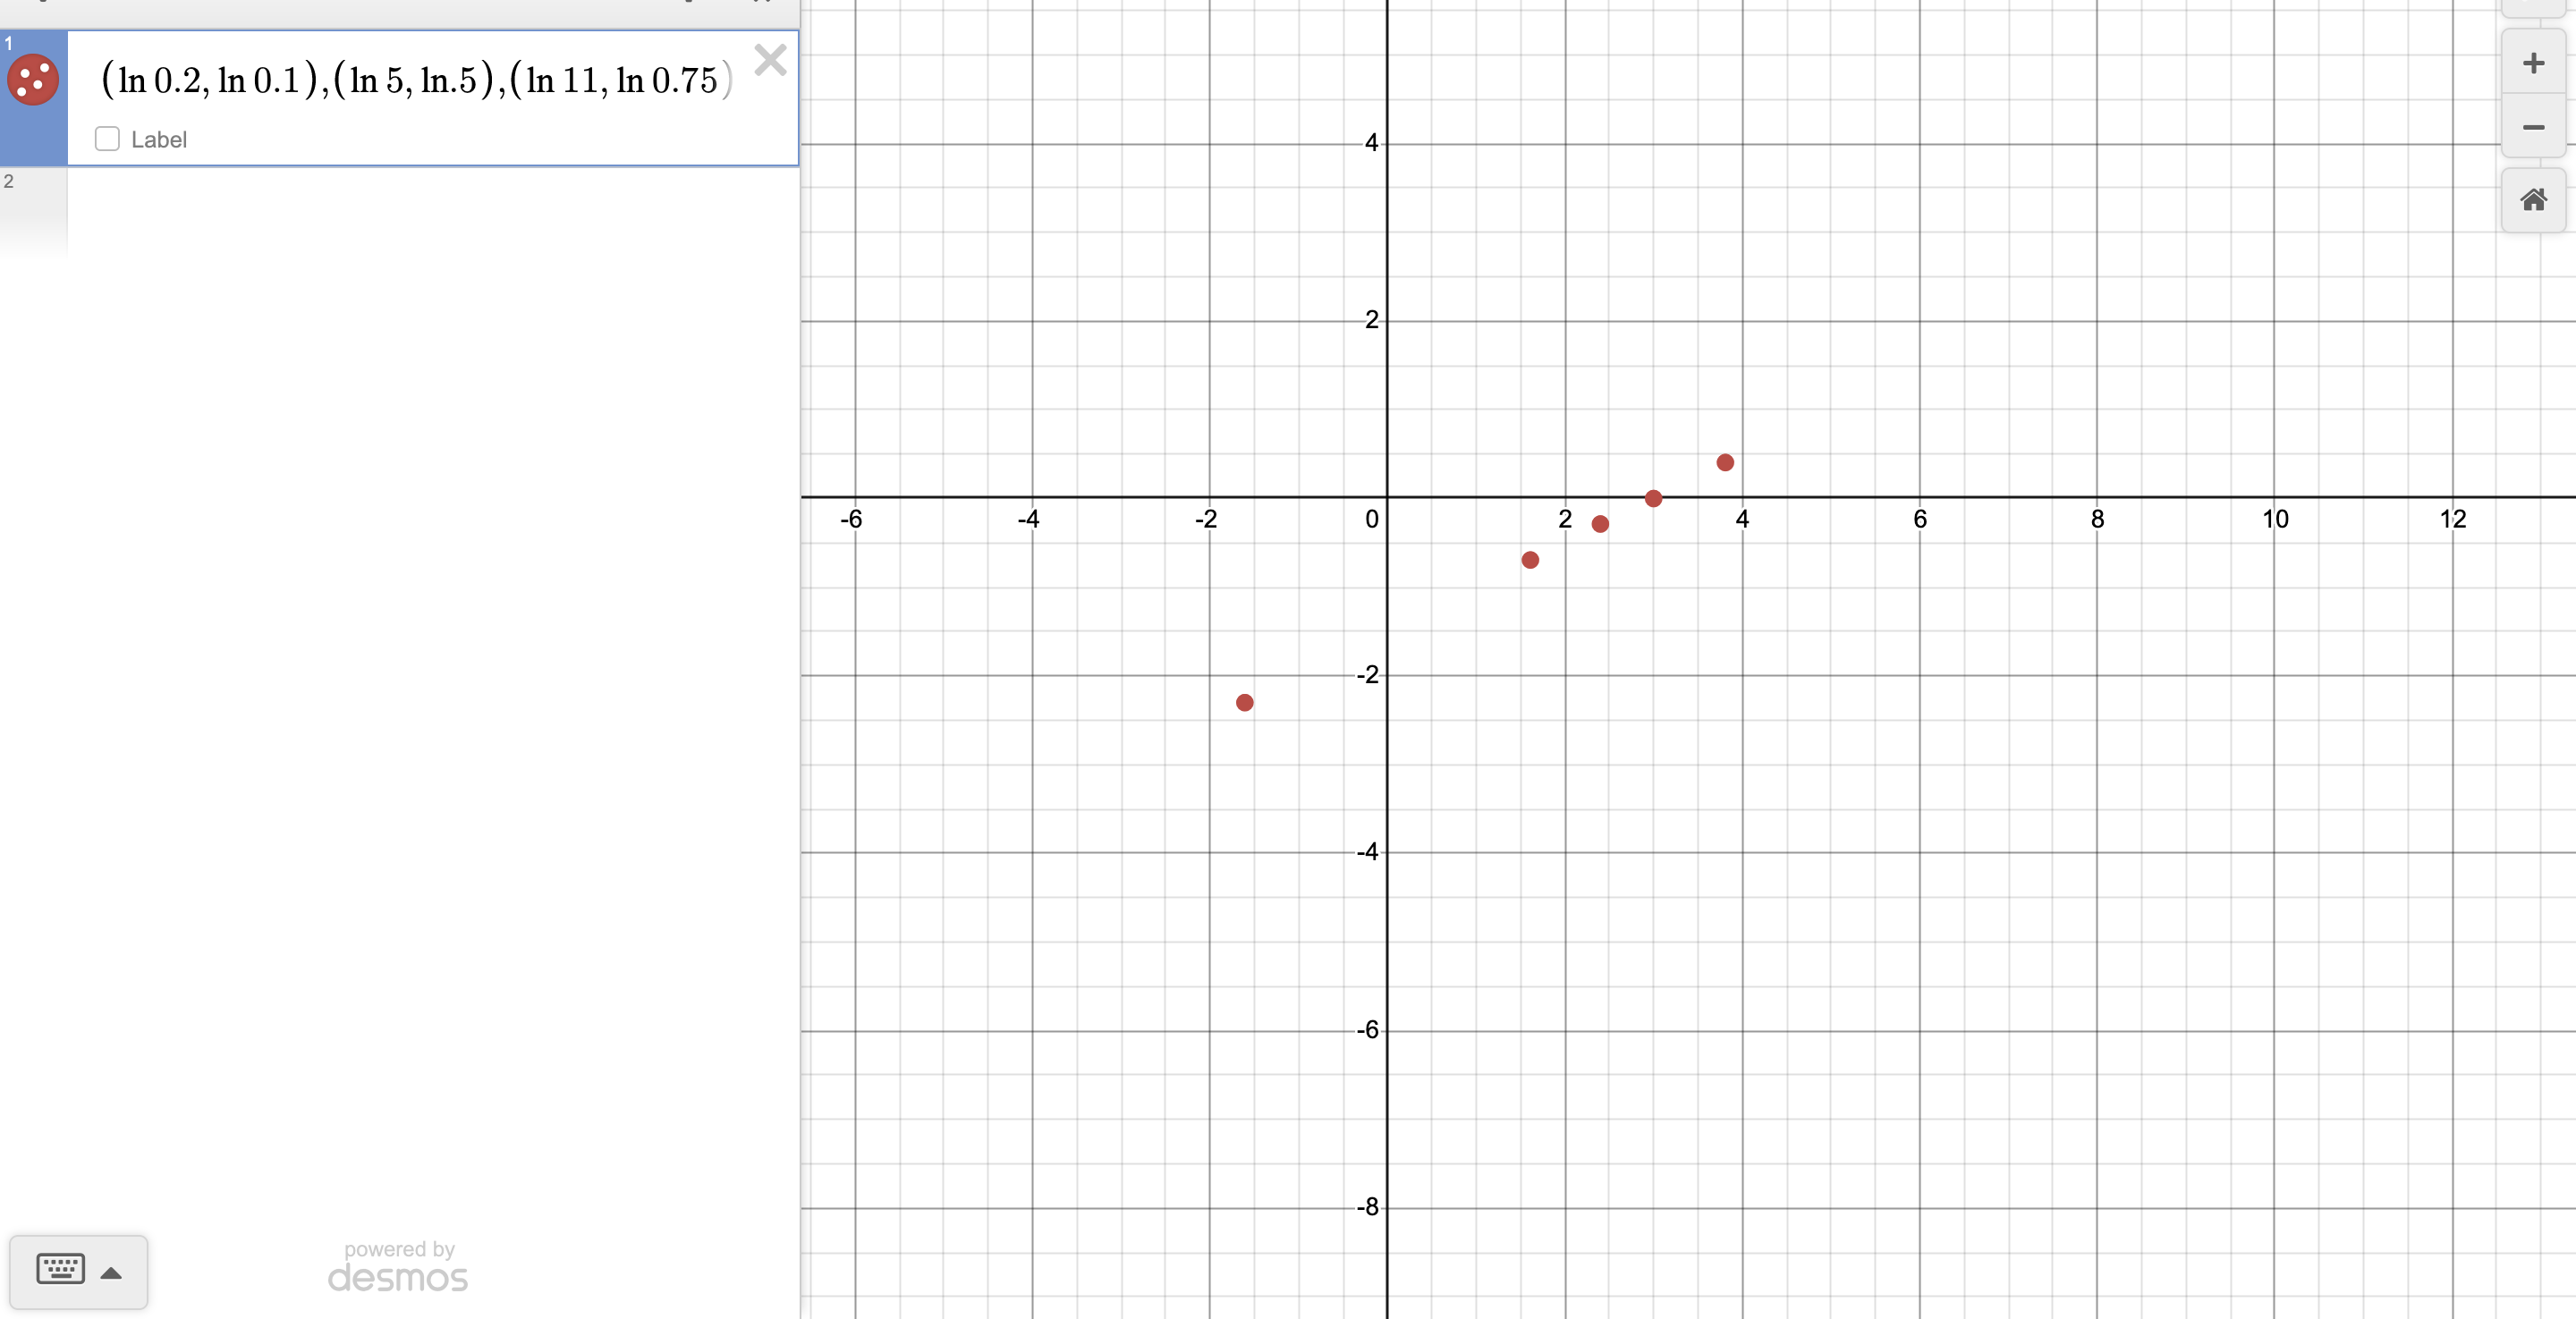
\includegraphics[width = 4in, height = 4in]{29} 


(b): From the scatter plot, it appears that the data is linear. Thus, we can predict that the slope would be:
\[ \frac{\ln 0.1-\ln 1.5}{\ln 0.2-\ln 45}=0.5 \]
meaning an equation to represent the linear data would be:
\[ \ln y-\ln 0.1=0.5(\ln x-\ln 0.2) \] and we can find the power function matching this data:
\[ \ln y-\ln 0.1=0.5(\ln x-\ln 0.2) \] \[ \ln y=0.5\ln x-1.498 \] \[ y=e^{0.5\ln x-1.498} \] \[ y\approx 0.224\times (x)^{0.5} \]
meaning the approximate speed of the current if the diameter was 120 milimeters would be:
\[ 0.224\times (120)^{0.5}\approx 2.454 \] meters per second.

\end{document}
